\chapter{Kiến trúc ứng dụng Android}
\label{chap:Chap}
Chương này trình bày tổng quan về kiến trúc ứng dụng Android từ tầng nền tảng hệ điều hành đến cách tổ chức và thực thi ứng dụng. Android được xây dựng trên nhân Linux, tận dụng các đặc tính như mã nguồn mở, khả năng quản lý tiến trình, bộ nhớ và bảo mật tốt. Hệ thống sử dụng cơ chế sandbox để cách ly ứng dụng thông qua UID riêng biệt, máy ảo(Dalvik hoặc ART) và hệ thống cấp quyền truy cập chặt chẽ. Các ứng dụng Android được đóng gói dưới dạng tệp APK, chứa mã bytecode(.dex), tài nguyên, cấu hình và chữ ký số. File AndroidManifest.xml đóng vai trò trung tâm trong việc khai báo quyền, cấu hình ứng dụng và các thành phần như Activity, Service, BroadcastReceiver và ContentProvider. Bên cạnh đó, Android hỗ trợ chia sẻ dữ liệu giữa các ứng dụng thông qua các cơ chế an toàn như ContentProvider, Intent hoặc FileProvider. Hệ thống cũng cho phép sử dụng các tính năng của Java 8 thông qua quá trình desugaring trong Gradle và công cụ D8/R8. Cuối cùng, chương đã đề cập đến các cải tiến và cơ chế bổ sung mà Google tích hợp vào nhân Linux như Binder, WakeLocks, SEAndroid để tối ưu cho môi trường di động. Qua đó, có thể thấy kiến trúc Android được thiết kế với mục tiêu tối ưu hóa hiệu suất, tăng tính bảo mật và cung cấp một nền tảng phát triển linh hoạt, mạnh mẽ cho các ứng dụng di động.

\section{Tổng quan về kiến trúc ứng dụng Android}
    % 1.1.
    \subsection{Các ngôn ngữ lập trình sử dụng (Java, các công nghệ đa nền tảng)}
    \renewcommand{\labelitemi}{--}    
    \begin{flushleft}
            \hspace*{0.8cm}Ngôn ngữ lập trình Android là tập hợp các ngôn ngữ được sử dụng để viết ứng dụng cho hệ điều hành Android. Hệ điều hành này phổ biến nhất trên thế giới, với hơn 2 tỷ thiết bị đang hoạt động. Với Android Studio là môi trường phát triển tích hợp chính thức từ Google, việc lập trình ứng dụng Android trở nên dễ dàng hơn bao giờ hết. Ngôn ngữ lập trình Android không chỉ là công cụ để xây dựng các ứng dụng di động phức tạp, mà còn mở ra cơ hội cho các nhà phát triển tạo ra các trải nghiệm đa dạng, từ ứng dụng doanh nghiệp đến trò chơi giải trí độc đáo.
    \end{flushleft}

    \begin{flushleft}
        \hspace*{0.8cm}Các ngôn ngữ lập trình phổ biến nhất cho việc phát triển ứng dụng Android hiện nay:
        \setlength{\leftmargini}{1.5cm}
        \begin{itemize}
            \item Java: Java đã là ngôn ngữ lập trình chính cho Android từ những ngày đầu của nền tảng này. Với cộng đồng lập trình viên lớn và nhiều tài liệu hỗ trợ, Java vẫn là một trong những lựa chọn hàng đầu cho việc phát triển ứng dụng Android.\\
            Ví dụ các ứng dụng đang sử dụng Java : Facebook, WhatApps,…
            \item Kotlin: Kotlin là ngôn ngữ có độ phổ biến ngày càng tăng cho việc phát triển ứng dụng Android. Kotlin cung cấp các tính năng hiện đại và làm cho việc viết mã dễ dàng hơn so với Java. Với sự ủng hộ mạnh mẽ từ Google, Kotlin đang trở thành ngôn ngữ lập trình được ưa chuộng nhất cho Android.\\
            Ví dụ các ứng dụng đang sử dụng Kotlin : Pinterest, Trello,…
            \item Dart: Dart là ngôn ngữ lập trình được sử dụng với framework Flutter – một công nghệ do Google phát triển để xây dựng ứng dụng đa nền tảng (Android, iOS, web, desktop). Dart cho phép lập trình viên viết một lần và triển khai trên nhiều nền tảng, với hiệu suất cao và giao diện người dùng đẹp mắt.\\
            Ví dụ các ứng dụng đang sử dụng Dart (với Flutter): Google Ads, Alibaba, Reflectly,…
        \end{itemize}
    \end{flushleft}

    \begin{flushleft}
        \hspace*{0.8cm}Việc lựa chọn ngôn ngữ lập trình nào để phát triển ứng dụng Android phụ thuộc vào nhiều yếu tố, bao gồm:
        \setlength{\leftmargini}{1.5cm}
        \begin{itemize}
            \item Kinh nghiệm và sở thích của lập trình viên: Nếu bạn đã có kinh nghiệm với Java hoặc Kotlin, bạn có thể sử dụng ngôn ngữ đó để phát triển ứng dụng Android. Nếu bạn mới bắt đầu học lập trình Android, Kotlin có thể là lựa chọn tốt hơn vì nó dễ học hơn Java.
            \item Loại ứng dụng bạn muốn phát triển: Một số ngôn ngữ lập trình phù hợp hơn với các loại ứng dụng nhất định. Ví dụ, C++ là lựa chọn tốt cho các trò chơi, trong khi Python là lựa chọn tốt cho các ứng dụng đơn giản.
            \item Mục tiêu phát triển: Phát triển nhanh(Python, Kotlin), hiệu suất cao(C++), Bảo trì dễ dàng(Java, Kotlin).
            \item Xu hướng thị trường: Kotlin là ngôn ngữ được Google khuyến khích sử dụng cho phát triển ứng dụng Android và đang dần trở nên phổ biến nhờ cú pháp hiện đại và khả năng tương thích tốt. Bên cạnh đó Java vẫn giữ vị trí là ngôn ngữ phổ biến nhất cho Android, tuy nhiên đang dần được thay thế bởi Kotlin trong nhiều dự án mới. Tiếp theo, C++ thường được sử dụng cho các ứng dụng đòi hỏi hiệu suất cao, như game hoặc xử lý đồ họa, nhưng không phổ biến bằng Java hay Kotlin. Trong khi đó, Python ít được sử dụng cho Android do hạn chế về hiệu suất và hỗ trợ nền tảng, tuy nhiên vẫn có thể phù hợp với các ứng dụng đơn giản hoặc phục vụ mục đích học tập, thử nghiệm.        
            \item Hỗ trợ từ cộng đồng: Các ngôn ngữ lập trình phổ biến hơn có cộng đồng hỗ trợ lớn hơn, giúp bạn dễ dàng tìm kiếm trợ giúp khi gặp khó khăn.   
        \end{itemize}
    \end{flushleft}

    % 1.2.
    \subsection{File APK và quá trình đưa ứng dụng lên Google Play, App Store}
    \renewcommand{\labelitemi}{--}
    \begin{flushleft}
        \hspace*{0.8cm}APK (Android Package) là định dạng tập tin được sử dụng để phân phối và cài đặt ứng dụng trên hệ điều hành Android, có đuôi mở rộng .apk, tương tự như .exe trong Windows hoặc .ipa trong IOS. Là gói nén chứa toàn bộ tài nguyên và mã thực thi của ứng dụng.\\
        Cấu trúc bên trong một file APK
        \begin{figure}[H] 
            \centering
            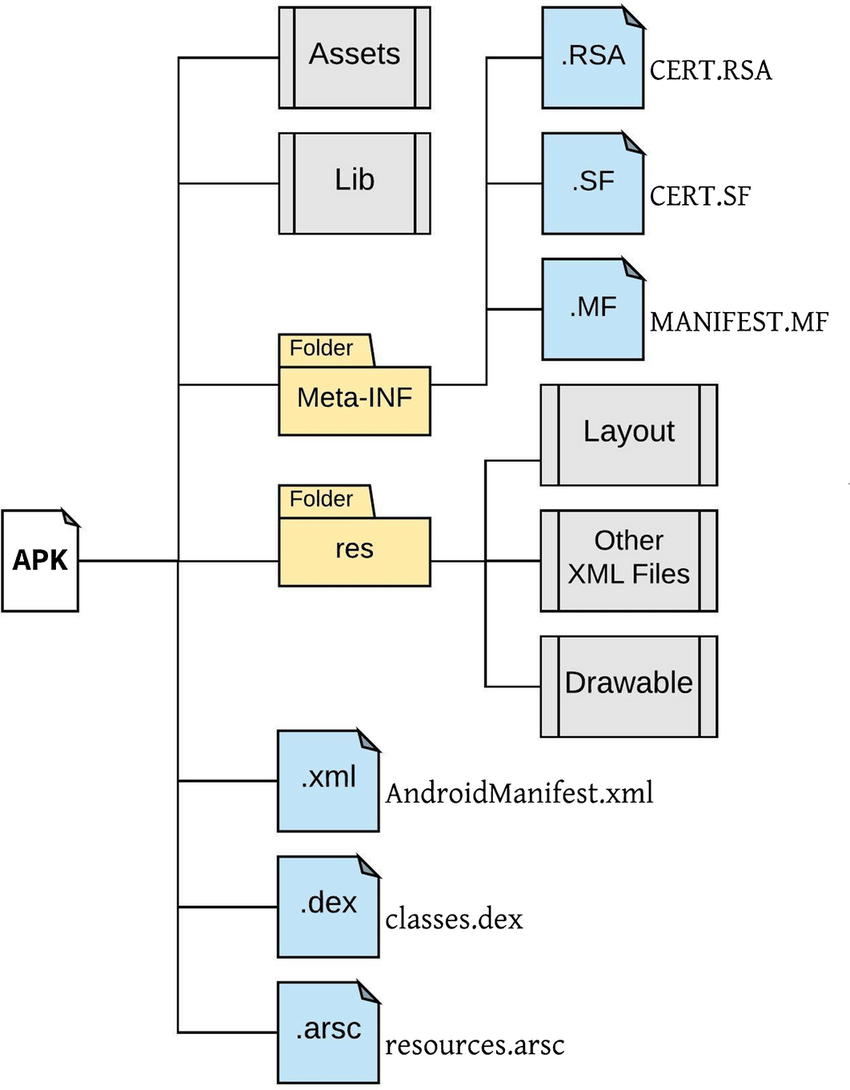
\includegraphics[width=0.5\textwidth]{images/apk.png}
            \caption{Cấu trúc file APK}
            \label{fig:android}
        \end{figure}
        
        \begin{table}[H]
            \centering
            \renewcommand{\arraystretch}{1.5}
            \begin{tabular}{|l|p{11cm}|}
                \hline
                \textbf{Thành phần} & \textbf{Mô tả} \\
                \hline
                \texttt{AndroidManifest.xml} & Chứa thông tin cấu hình ứng dụng: tên gói, phiên bản, các quyền truy cập, khai báo thành phần như Activity, Service, Receiver... \\
                \hline
                \texttt{classes.dex} & Chứa mã bytecode đã được biên dịch từ mã nguồn Java hoặc Kotlin. Đây là phần chính được thực thi trong máy ảo Dalvik hoặc ART. \\
                \hline
                \texttt{resources.arsc} & Tập hợp các tài nguyên đã được biên dịch như chuỗi ký tự (string), style, màu sắc và các giá trị được lưu trong XML. \\
                \hline
                \texttt{res/} & Thư mục chứa các tài nguyên chưa biên dịch như hình ảnh, layout XML, drawable, v.v. \\
                \hline
                \texttt{lib/} & Thư mục chứa các thư viện native (viết bằng C/C++) tương ứng với từng kiến trúc CPU (như ARM, x86...). \\
                \hline
                \texttt{META-INF/} & Lưu trữ các tệp liên quan đến chứng chỉ số, thông tin chữ ký APK để xác thực và bảo vệ toàn vẹn nội dung. \\
                \hline
                \texttt{assets/} & Chứa các tài nguyên thô (raw) do lập trình viên thêm vào, có thể truy cập qua `AssetManager`. \\
                \hline
            \end{tabular}
            \caption{Cấu trúc các thành phần bên trong file APK}
            \label{table:apk-structure}
            \end{table}            
    
        \hspace*{0.8cm}Quy trình khi đưa ứng dụng lên Google Play:  \\
        \setlength{\parskip}{1em}\hspace*{0.6cm}Build APK, từ mã nguồn Android (bằng Android Studio), tạo ra file .apk. Ký số (Signing), ứng dụng được ký bằng private key để xác thực nguồn gốc. Upload lên Google Play, Google kiểm tra, và nếu muốn, có thể dùng App Signing by Google Play, là dịch vụ Google giữ private key. Phân phối và cài đặt, người dùng tải về và cài đặt ứng dụng trực tiếp từ APK.\\

        \hspace*{0.8cm}Tóm lại APK là đơn vị triển khai duy nhất trên Android, có thể chia sẻ trực tiếp (qua web, Bluetooth, email…) mà không cần qua Play Store, dễ dàng trích xuất hoặc phân tích để debug hoặc reverse engineering (nên phải cẩn thận bảo vệ mã nguồn).
    \end{flushleft}

\section{Cơ chế hoạt động của hệ điều hành Android}

% 2.1
\subsection{Android trên nền tảng Linux}
\renewcommand{\labelitemi}{--}    
\begin{flushleft}
    \hspace*{0.8cm}Android được xây dựng trên nhân (kernel) của hệ điều hành Linux, tức là sử dụng Linux kernel làm lớp điều khiển phần cứng như quản lý bộ nhớ, tiến trình, thiết bị ngoại vi và bảo mật hệ thống. Trong khi đó, các thành phần còn lại như giao diện người dùng, framework ứng dụng và dịch vụ hệ thống đều do Google phát triển riêng biệt, không sử dụng giao diện truyền thống của Linux. Android chọn Linux kernel vì đây là nền tảng mã nguồn mở, ổn định, có tính bảo mật cao và hỗ trợ tốt cho các tính năng quan trọng của thiết bị di động như xử lý đa tiến trình, cấp quyền truy cập theo người dùng và hỗ trợ phần cứng đa dạng. Việc kế thừa nhân Linux giúp Android tăng tính linh hoạt, tiết kiệm thời gian phát triển và dễ dàng tùy biến cho từng nhà sản xuất thiết bị.\\
    \newpage
    Google đã tùy biến kernel Linux để phù hợp hơn với điện thoại:
    \begin{table}[H]
        \centering
        \renewcommand{\arraystretch}{1.5}
        \begin{tabular}{|p{3.5cm}|p{12cm}|}
            \hline
            \textbf{Tính năng bổ sung} & \textbf{Công dụng} \\
            \hline
            WakeLocks & Cho phép ứng dụng hoặc hệ thống giữ CPU không rơi vào trạng thái ngủ khi cần thực hiện các tác vụ nền quan trọng, giúp tiết kiệm pin một cách chủ động. \\
            \hline
            Ashmem  & Cung cấp cơ chế chia sẻ vùng nhớ tạm thời giữa các tiến trình, cho phép truyền dữ liệu hiệu quả mà không cần lưu vào bộ nhớ lâu dài. \\
            \hline
            Binder IPC & Là hệ thống giao tiếp liên tiến trình (Inter-Process Communication) do Android phát triển, dùng để truyền dữ liệu và lệnh giữa các app và dịch vụ hệ thống một cách an toàn và nhanh chóng. \\
            \hline
            Logger & Ghi lại thông tin log hệ thống, giúp nhà phát triển theo dõi, phân tích lỗi và hoạt động của ứng dụng hoặc hệ điều hành. \\
            \hline
            Alarm Drivers & Quản lý các sự kiện báo thức (alarm) trong hệ thống, cho phép ứng dụng thực thi tác vụ định kỳ hoặc vào một thời điểm nhất định, kể cả khi thiết bị đang ở trạng thái nghỉ. \\
            \hline
        \end{tabular}
        \caption{Các tính năng bổ sung do Google thêm vào Linux để hỗ trợ hệ điều hành Android}
        \label{table:android-linux-features}
        \end{table}          
\end{flushleft}

\renewcommand{\labelitemi}{--}    
    \begin{flushleft}
        \hspace*{0.8cm}Mỗi ứng dụng gắn với một định danh người dùng riêng. UID (User ID) là mã định danh người dùng cấp hệ điều hành. Trong Android, mỗi ứng dụng (app) được xem như một người dùng độc lập, và hệ thống cấp cho nó một UID riêng biệt.
        \setlength{\leftmargini}{1.5cm}
        \begin{itemize}
            \item Nguồn gốc UID: Android dựa trên Linux kernel, và Linux có mô hình đa người dùng. Mỗi tiến trình (process) trong Linux chạy dưới quyền của một user cụ thể, phân biệt bằng UID.Android tận dụng mô hình này để tăng tính bảo mật cho các ứng dụng.
            \item Mỗi app có vùng dữ liệu riêng (trong /data/data/<tên gói>) mà chỉ UID đó mới truy cập được. Không app nào có thể truy cập trực tiếp vào dữ liệu của app khác, trừ khi quyền được cấp thông qua hệ thống permission và kiểm soát quyền truy cập tập tin, cơ sở dữ liệu, socket. Ghi log và debug app. Cấp phép hoặc từ chối quyền (ví dụ camera, GPS...), do đó UID rất quan trọng.
        \end{itemize}

        \begin{figure}[H] 
            \centering
            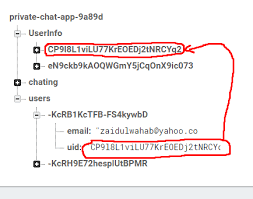
\includegraphics[width=0.5\textwidth]{images/uid.png}
            \caption{Ví dụ về cấu trúc lưu trữ người dùng và thông tin trò chuyện}
            \label{fig:android}
        \end{figure}
    \end{flushleft}

% 2.2
\subsection{Cơ chế sandbox}
\renewcommand{\labelitemi}{--}    
    \begin{flushleft}
        \hspace*{0.8cm}Sandbox trong Android là một môi trường cách ly, nơi mỗi ứng dụng (app) được “nhốt” vào một không gian riêng biệt, không thể trực tiếp can thiệp hay truy cập vào dữ liệu hoặc tiến trình của ứng dụng khác. Hình dung như mỗi app sống trong một “phòng riêng” với cửa khóa, không ai ra vào nếu không có chìa khóa (quyền được cấp).\\
        \setlength{\leftmargini}{1.5cm}
        \hspace*{0.8cm}Cách Android thực hiện sandbox: kết hợp nhiều công nghệ
        \begin{table}[H]
            \centering
            \renewcommand{\arraystretch}{1.5}
            \begin{tabular}{|p{4.5cm}|p{11cm}|}
                \hline
                \textbf{Cơ chế bảo mật} & \textbf{Mục đích} \\
                \hline
                UID riêng biệt cho mỗi app & Mỗi ứng dụng được gán một mã định danh người dùng (UID) riêng biệt, giúp chạy như một "user" độc lập trên nền tảng Linux, cách ly tài nguyên giữa các ứng dụng. \\
                \hline
                Filesystem permissions & Quyền truy cập hệ thống tệp tin được kiểm soát để mỗi ứng dụng chỉ có thể truy cập vào vùng dữ liệu riêng của nó, chẳng hạn như thư mục `/data/data/com.example.app`. \\
                \hline
                Máy ảo (VM) & Mỗi ứng dụng chạy trong một máy ảo riêng (trước đây là Dalvik, hiện tại là ART), giúp cách ly mã thực thi và tăng tính an toàn khi xử lý mã bytecode. \\
                \hline
                Permission system & Nếu ứng dụng muốn truy cập các tài nguyên hệ thống ngoài vùng sandbox như camera, GPS, microphone, hệ thống sẽ yêu cầu xin quyền rõ ràng từ người dùng. \\
                \hline
                SEAndroid & Dựa trên SELinux, SEAndroid bổ sung chính sách bảo mật ở cấp nhân hệ điều hành, kiểm soát hành vi truy cập tài nguyên của từng ứng dụng theo nguyên tắc tối thiểu quyền. \\
                \hline
            \end{tabular}
            \caption{Các cơ chế trong Android đảm bảo môi trường sandbox cho mỗi ứng dụng}
            \label{table:android-sandbox-mechanisms}
            \end{table}
            
    \end{flushleft}

    \begin{flushleft}
      \hspace*{0.8cm}Sandbox bảo vệ những thứ sau:
      \setlength{\leftmargini}{1.5cm}
      \begin{itemize}
          \item Dữ liệu app(database, file, cache...): Không app nào khác có thể truy cập nếu không được cấp quyền
            \item Mã nguồn (classes.dex): Không bị sửa đổi/thay thế bởi app khác
            \item Giao tiếp giữa app: Chỉ có thể qua các cơ chế an toàn như Intent, ContentProvider, Binder
            \item Tài nguyên hệ thống (camera, GPS, v.v.): Chỉ truy cập được nếu người dùng cho phép thông qua hệ thống permission
        \end{itemize}
        \hspace*{0.8cm}Ví dụ: Giả sử có 2 app:
        App1 là ghi chú cá nhân,
        App2 là trò chơi.
        Cơ chế bảo vệ làm cho App2 không thể đọc được ghi chú của App1, trừ khi App1 cung cấp dữ liệu qua Intent, ContentProvider\\
        \hspace*{0.8cm}Tóm lại, Sandbox là lá chắn vô hình bảo vệ mỗi ứng dụng Android như một thế giới riêng biệt. Nó giúp người dùng yên tâm cài đặt nhiều ứng dụng mà không sợ bị can thiệp trái phép
  \end{flushleft}

% 2.3
\subsection{Máy ảo (VM) riêng cho mỗi ứng dụng}

\begin{flushleft}
  \hspace*{0.8cm}Máy ảo là một chương trình mô phỏng một hệ thống máy tính khác, cho phép chạy phần mềm như thể đang chạy trực tiếp trên một máy vật lý. Máy ảo không tương tác trực tiếp với phần cứng, mà thay vào đó hoạt động như một lớp trung gian giữa phần mềm và phần cứng thật. Mỗi máy ảo có môi trường thực thi riêng biệt, được cách ly hoàn toàn, giúp đảm bảo an toàn, ổn định và khả năng quản lý tài nguyên hiệu quả. Trong Android, máy ảo (cụ thể là Dalvik VM hoặc Android Runtime – ART) giữ vai trò trung gian để chạy các ứng dụng Android được biên dịch dưới dạng bytecode. Mã bytecode này được đóng gói trong tệp .dex, và là thành phần quan trọng nằm trong gói cài đặt ứng dụng .apk. Nhờ máy ảo, các ứng dụng có thể được chạy một cách độc lập, không ảnh hưởng đến các ứng dụng khác và bị giới hạn trong vùng tài nguyên mà hệ điều hành cho phép, giúp thực hiện cơ chế sandbox hiệu quả. Máy ảo cũng là yếu tố giúp hệ thống có khả năng phát hiện, cô lập lỗi và ngăn chặn hành vi xâm nhập không mong muốn từ ứng dụng độc hại.
\end{flushleft}

\begin{flushleft}
  \hspace*{0.8cm}Dalvik VM ($Android \leq 4.x$): Là máy ảo đầu tiên của Android,  được thiết kế để chạy các ứng dụng Android trên các thiết bị di động với tài nguyên hạn chế. Dalvik sử dụng register-based architecture, khác với các máy ảo khác như Java Virtual Machine (JVM) vốn dựa trên stack-based architecture. Điều này có nghĩa là phần lớn các phép toán trong Dalvik được thực hiện trên các thanh ghi thay vì bộ nhớ, giúp giảm độ phức tạp và tối ưu hóa hiệu suất. Dalvik còn sử dụng Just-In-Time (JIT) compilation, nghĩa là mã ứng dụng được biên dịch thành mã máy khi ứng dụng đang chạy, thay vì biên dịch toàn bộ trước khi cài đặt. Điều này giúp tiết kiệm bộ nhớ và rút ngắn thời gian cài đặt ứng dụng, vì không cần biên dịch mã trước khi triển khai. Tuy nhiên, Dalvik cũng có một số nhược điểm. Quá trình khởi động ứng dụng có thể bị chậm vì mã phải được biên dịch khi chạy, dẫn đến trải nghiệm người dùng không mượt mà. Bên cạnh đó, hiệu suất tổng thể của Dalvik cũng không cao bằng các máy ảo khác, vì việc biên dịch mã trong thời gian chạy có thể gây ra sự chậm trễ trong quá trình thực thi ứng dụng. Mặc dù vậy, Dalvik vẫn là nền tảng quan trọng trong sự phát triển của Android cho đến khi được thay thế bởi ART (Android Runtime) trong các phiên bản Android sau này.
  Dùng từ Android 1.0 đến Android 4.4 (KitKat).
  \begin{figure}[H] 
    \centering
    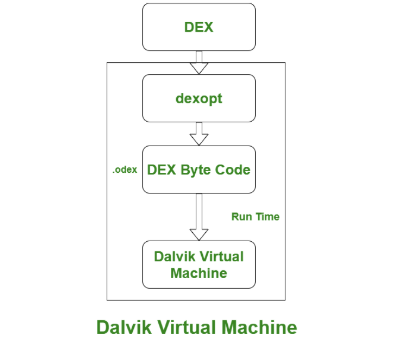
\includegraphics[width=0.6\textwidth]{images/DalvikVM.png}
    \caption{Máy ảo Dalvik}
    \label{fig:android}
\end{figure}  
\end{flushleft}

\begin{flushleft}
    \hspace*{0.8cm}ART (Android Runtime): Thay thế Dalvik từ Android 5.0 (Lollipop), dùng AOT (Ahead-Of-Time) compilation để mã được biên dịch thành mã máy ngay khi cài app.
    Lợi ích là khởi chạy nhanh, hiệu suất cao.
    Nhược điểm là cài đặt lâu hơn, chiếm nhiều bộ nhớ.
    Sau Android 7.0, ART còn hỗ trợ thêm JIT lẫn AOT do đó tối ưu thời gian chạy lẫn bộ nhớ.   
    \begin{figure}[H] 
        \centering
        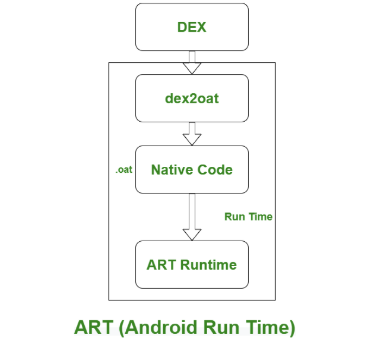
\includegraphics[width=0.6\textwidth]{images/ART.png}
        \caption{Android Run Time}
        \label{fig:android}
    \end{figure}  
\end{flushleft}

\begin{flushleft}
    \hspace*{0.8cm}Quy trình thực thi của Dalvik VM và ART:
    \begin{table}[H]
        \centering
        \renewcommand{\arraystretch}{1.5}
        \begin{tabular}{|p{4cm}|p{5cm}|p{5cm}|}
        \hline
        \textbf{Giai đoạn} & \textbf{Dalvik VM} & \textbf{ART (Android Runtime)} \\
        \hline
        Khi cài đặt ứng dụng & Chép file \texttt{.dex} vào hệ thống & Biên dịch \texttt{.dex} thành mã máy \texttt{.oat} \\
        \hline
        Khi chạy ứng dụng & Dịch bytecode thành mã máy trong thời gian thực (JIT) & Chạy mã máy đã được biên dịch sẵn (AOT) \\
        \hline
        Khi mở lại ứng dụng & Vẫn phải dịch lại bytecode & Khởi động rất nhanh, không cần biên dịch lại \\
        \hline
        \end{tabular}
        \caption{So sánh quá trình thực thi ứng dụng giữa Dalvik VM và ART}
        \label{tab:dalvik-vs-art}
        \end{table}
          
    \hspace*{0.8cm} Lý do Google chuyển từ Dalvik sang ART: Hiệu suất tăng mạnh (app khởi động nhanh hơn), tiết kiệm pin hơn, tối ưu RAM và bộ nhớ tốt hơn, chuẩn bị cho tương lai với các công nghệ như: Android Instant Apps, Dynamic Delivery
\end{flushleft}

\renewcommand{\labelitemi}{--}    
    \begin{flushleft}
        \hspace*{0.8cm}Mỗi ứng dụng là một tiến trình độc lập. Trong Android, mỗi ứng dụng (app) khi được khởi chạy sẽ được cấp phát một tiến trình riêng biệt (process). Tiến trình này có vùng nhớ riêng, UID riêng, máy ảo riêng, hoạt động độc lập, không can thiệp lẫn nhau.
    \end{flushleft}
\newpage
    \begin{flushleft}
      \setlength{\leftmargini}{1.5cm}
      \begin{itemize}
        \item Lợi ích: App không thể truy cập dữ liệu, bộ nhớ hay tiến trình của app khác (bảo mật), nếu 1 app lag/crash, không ảnh hưởng app khác(tối ưu hiệu năng), có thể theo dõi, dừng, hoặc khởi động lại tiến trình một cách riêng lẻ(quản lí tài nguyên), khi hệ thống cần RAM, Android có thể tắt tiến trình app ít dùng mà không ảnh hưởng toàn hệ thống(tự động giải phóng)
        \item Android tạo ra một tiến trình mới: khi người dùng mở ứng dụng lần đầu, app được khởi động lại sau khi bị hệ thống giải phóng
        \item Vùng nhớ riêng trong mỗi tiến trình: mỗi tiến trình chỉ "thấy" được biến, đối tượng trong phạm vi của nó, dữ liệu trong thư mục app, không thể trực tiếp truy cập đến vùng nhớ của tiến trình khác (do cơ chế sandbox, UID, VM kết hợp bảo vệ).
      \end{itemize}
    \end{flushleft}

\section{Chia sẻ dữ liệu giữa các ứng dụng}

\begin{flushleft}
  \hspace*{0.8cm}Trong hệ điều hành Android, mỗi ứng dụng khi được cài đặt sẽ hoạt động như một thực thể độc lập, được bảo vệ bằng cơ chế sandbox. Cơ chế này ngăn cản ứng dụng truy cập trực tiếp vào dữ liệu của ứng dụng khác, giúp nâng cao tính bảo mật và quyền riêng tư cho người dùng. Tuy nhiên, trong một số tình huống thực tế, các ứng dụng vẫn cần khả năng chia sẻ dữ liệu cho nhau. Ví dụ, một ứng dụng chỉnh sửa ảnh có thể cần truy cập đến bộ sưu tập ảnh, hoặc một ứng dụng mạng xã hội cần truy cập danh bạ để đề xuất kết bạn. Để hỗ trợ nhu cầu này mà vẫn đảm bảo an toàn, Android cung cấp một số cơ chế chuẩn để chia sẻ dữ liệu giữa các ứng dụng một cách kiểm soát và có chọn lọc.
\end{flushleft}

% 3.1
\subsection{Cơ chế dùng chung User-id}
\renewcommand{\labelitemi}{--}    
    \begin{flushleft}
        \hspace*{0.8cm}Đây là một điểm trong bảo mật và cấp quyền của Android Các ứng dụng Android có thể dùng chung user-id nếu có cùng chứng chỉ số (digital certificate)
        \setlength{\leftmargini}{1.5cm}
        \begin{itemize}
            \item Mặc định khi một ứng dụng được cài đặt, hệ điều hành Android sẽ tạo một UID (User ID) riêng biệt cho nó, mỗi app chỉ có thể truy cập tài nguyên của chính nó (sandbox).
            \item Hai hoặc nhiều ứng dụng có thể dùng chung UID nếu chúng được ký bằng cùng một khóa chứng thực số (digital certificate) và chúng khai báo "android:sharedUserId" giống nhau trong AndroidManifest.xml
            \item Yêu cầu bắt buộc là chứng chỉ số giống nhau, Android dùng digital signature để đảm bảo chỉ các app thuộc cùng một nhà phát triển mới có thể chia sẻ UID. Điều này ngăn chặn app lạ cố tình khai báo sharedUserId để xâm nhập dữ liệu của app khác.
            Ví dụ nếu app A và app B có sharedUserId giống nhau nhưng ký bằng chứng chỉ khác nhau → Hệ thống từ chối cài đặt!
            \item Lợi ích là các app có thể truy cập dữ liệu và file của nhau, có thể dùng chung database, file cấu hình…, có thể chia sẻ quyền như đọc SMS, camera… nếu quyền được cấp
        \end{itemize}
    \end{flushleft}

% 3.2
\subsection{ContentProvider và Intent}    
    \begin{flushleft}
        \hspace*{0.8cm}Một trong những cơ chế chia sẻ dữ liệu quan trọng nhất trong Android là ContentProvider. Đây là một lớp trung gian cho phép một ứng dụng cung cấp quyền truy cập có kiểm soát đến dữ liệu của mình cho các ứng dụng khác. ContentProvider hoạt động giống như một cơ sở dữ liệu với API chuẩn, cho phép các ứng dụng khác thực hiện thao tác như đọc, ghi, sửa hoặc xóa thông tin, nhưng chỉ trong phạm vi mà nhà phát triển cho phép. Ví dụ điển hình là ứng dụng Danh bạ của Android – nó triển khai một ContentProvider cho phép các ứng dụng khác như Zalo, Facebook hay Viber truy xuất thông tin liên lạc, nhưng chỉ sau khi người dùng đồng ý cấp quyền.\\
        \hspace*{0.8cm}Ngoài ContentProvider, Android còn hỗ trợ chia sẻ dữ liệu thông qua các Intent. Intent là một cơ chế giao tiếp giữa các thành phần trong Android, có thể được sử dụng để truyền dữ liệu giữa các Activity, Service, hoặc giữa các ứng dụng khác nhau. Khi một ứng dụng muốn gửi một tập tin, một đoạn văn bản, hình ảnh hoặc bất kỳ dữ liệu nào sang ứng dụng khác (ví dụ như chia sẻ ảnh lên mạng xã hội), nó có thể tạo một Intent có chứa dữ liệu và gọi startActivity hoặc startActivityForResult. Ứng dụng nhận dữ liệu sẽ phải khai báo rõ ràng trong AndroidManifest.xml các intent filter phù hợp để có thể tiếp nhận loại dữ liệu đó. Cơ chế này đơn giản, phổ biến, và rất hiệu quả cho các thao tác chia sẻ ngắn hạn, không yêu cầu truy cập thường xuyên.\\
        \hspace*{0.8cm}Một phương pháp khác nữa là sử dụng bộ nhớ ngoài (external storage), tức là các file được lưu trên thẻ nhớ hoặc phân vùng có thể truy cập công khai. Trước đây, bất kỳ ứng dụng nào có quyền đọc/ghi vào bộ nhớ ngoài đều có thể truy cập dữ liệu của ứng dụng khác lưu ở đó. Tuy nhiên, kể từ Android 10 (API 29), Google đã giới thiệu cơ chế Scoped Storage để hạn chế quyền truy cập tự do này. Scoped Storage yêu cầu ứng dụng chỉ có thể truy cập vào thư mục riêng của mình trên bộ nhớ ngoài hoặc các file cụ thể được chia sẻ thông qua MediaStore hoặc Storage Access Framework. Điều này đảm bảo rằng không có ứng dụng nào có thể âm thầm đọc hoặc ghi lên dữ liệu của ứng dụng khác mà không có sự cho phép rõ ràng.
    \end{flushleft}

% 3.3
\subsection{FileProvider}
\renewcommand{\labelitemi}{--}    
    \begin{flushleft}
        \hspace*{0.8cm}Một cách hiện đại và an toàn để chia sẻ dữ liệu giữa ứng dụng là sử dụng các API do hệ thống quản lý như FileProvider. Đây là một lớp đặc biệt giúp ứng dụng có thể chia sẻ tệp tin thông qua URI mà không cần cấp quyền truy cập bộ nhớ ngoài toàn cục. FileProvider chỉ cấp quyền truy cập tạm thời, đúng với tệp mà ứng dụng chia sẻ, và chỉ dành cho ứng dụng nhận cụ thể trong một khoảng thời gian nhất định. Điều này giúp tránh được việc ứng dụng khác có thể lén đọc toàn bộ dữ liệu người dùng mà không được cho phép.
    \end{flushleft}
    \begin{flushleft}
      \hspace*{0.8cm}$\Rightarrow$ Tóm lại, Android cung cấp nhiều phương thức để chia sẻ dữ liệu giữa các ứng dụng, mỗi phương thức phù hợp với từng nhu cầu khác nhau. Tuy nhiên, tất cả các cơ chế này đều được thiết kế với tiêu chí an toàn và bảo vệ quyền riêng tư người dùng. Việc chia sẻ dữ liệu phải luôn được thực hiện thông qua cơ chế kiểm soát, có sự đồng ý của người dùng, và hạn chế tối đa quyền truy cập không cần thiết. Trong thời điểm hiện tại, Google cũng khuyến khích các nhà phát triển di chuyển sang những cơ chế chia sẻ an toàn như FileProvider, ContentProvider hoặc sử dụng các API hệ thống để tương tác dữ liệu.
    \end{flushleft}

% 3.4
\subsection{Một số quyền truy cập phổ biến}
    \begin{flushleft}
        \hspace*{0.8cm}Trong quá trình phát triển ứng dụng Android, nhà phát triển thường cần truy cập đến các tài nguyên nhạy cảm trên thiết bị, và mỗi loại tài nguyên đều tương ứng với một hoặc nhiều quyền truy cập cụ thể mà ứng dụng cần khai báo trong file AndroidManifest.xml, đồng thời phải xin phép người dùng tại thời điểm chạy (runtime) nếu thuộc nhóm nguy hiểm. Ví dụ, để truy cập danh bạ người dùng, ứng dụng cần khai báo quyền android.permission.READ-CONTACTS. Đây là quyền nguy hiểm vì liên quan đến thông tin cá nhân, nên bắt buộc phải xin người dùng cho phép khi chạy ứng dụng.\\
        \hspace*{0.8cm}Tương tự, nếu ứng dụng cần gửi hoặc nhận tin nhắn SMS, nhà phát triển phải sử dụng các quyền như SEND-SMS, RECEIVE-SMS và READ-SMS. Đây là những quyền cực kỳ nhạy cảm, liên quan đến quyền riêng tư và chi phí tài chính của người dùng, nên Android yêu cầu phải có lý do rõ ràng và được người dùng cho phép rõ ràng tại runtime.\\
        \hspace*{0.8cm}Việc truy cập thông tin trạng thái thiết bị, như số IMEI hay tình trạng cuộc gọi, đòi hỏi quyền READ-PHONE-STATE. Tuy nhiên, kể từ Android 10, quyền này bị giới hạn mạnh và chỉ cho phép truy cập một số thông tin cơ bản, trừ khi ứng dụng được cấp quyền đặc biệt thông qua Google Play Console. Đối với thông tin vị trí, Android cung cấp hai loại quyền là ACCESS-FINE-LOCATION (vị trí chính xác qua GPS) và ACCESS-COARSE-LOCATION (vị trí tương đối qua mạng). Từ Android 10 trở đi, hệ thống yêu cầu người dùng phải xác định rõ ứng dụng có được quyền truy cập vị trí liên tục không, hay chỉ khi đang sử dụng.\\
        \hspace*{0.8cm}Truy cập vào phần cứng như camera và micro cũng cần xin quyền rõ ràng. Để sử dụng camera, ứng dụng cần có android.permission.CAMERA, và để ghi âm giọng nói, phải khai báo android.permission.RECORD-AUDIO. Cả hai quyền này đều được xếp vào nhóm quyền nhạy cảm, yêu cầu phải xin ở runtime và được người dùng cấp phép rõ ràng. Ngoài ra, để tăng tính minh bạch và tuân thủ chính sách Google Play, ứng dụng cũng nên thông báo trước cho người dùng về lý do cần các quyền này và cách chúng sẽ được sử dụng.
    \end{flushleft} 
\newpage

\section{Ưu điểm của việc sử dụng ngôn ngữ Java trong lập trình Android}
        Java là một trong những ngôn ngữ lập trình lâu đời và phổ biến nhất trên thế giới. Việc sử dụng Java trong lập trình Android giúp lập trình viên dễ dàng tiếp cận với nguồn tài nguyên phong phú từ tài liệu học tập, ví dụ thực tế đến sự hỗ trợ từ cộng đồng. Java sử dụng hệ thống kiểu dữ liệu chặt chẽ(strongly typed), giúp phát hiện lỗi cú pháp và logic ngay trong quá trình biên dịch. Điều này làm tăng độ an toàn của chương trình và giảm thiểu nguy cơ phát sinh lỗi trong quá trình thực thi.

        \vspace{0.5em}

        Một trong những triết lý cốt lõi của Java là “Write once, run anywhere” – nghĩa là mã nguồn chỉ cần viết một lần và có thể chạy trên nhiều nền tảng khác nhau mà không cần chỉnh sửa. Điều này có được là nhờ Java chạy trên máy ảo JVM, giúp mã được biên dịch thành bytecode độc lập với hệ điều hành. Khi lập trình Android bằng Java, điều này đồng nghĩa với việc bạn có thể dễ dàng tái sử dụng phần lớn mã nguồn cho các ứng dụng chạy trên nền tảng khác như desktop hoặc server-side Java.

        \vspace{0.5em}

        Hệ sinh thái phát triển rất phong phú với hàng loạt công cụ và thư viện hỗ trợ mạnh mẽ, tiêu biểu như Android Studio – môi trường phát triển chính thức cho Android. Ngoài ra, Gradle giúp tự động hóa quá trình build, còn hàng nghìn thư viện mã nguồn mở khác có thể giúp giảm đáng kể thời gian và công sức viết mã. Hơn nữa, cộng đồng lập trình viên Java rất đông đảo và hoạt động tích cực, giúp bạn dễ dàng tìm được câu trả lời cho các vấn đề kỹ thuật trên các diễn đàn như Stack Overflow, GitHub, hay cộng đồng Google Developer.

        \vspace{0.5em}

        Java hỗ trợ cơ chế quản lý bộ nhớ tự động thông qua trình thu gom rác(Garbage Collector). Thay vì phải tự giải phóng bộ nhớ như trong C hoặc C++, lập trình viên Java không cần lo lắng về việc quản lý tài nguyên thủ công. Trình thu gom rác sẽ tự động theo dõi và thu hồi vùng nhớ không còn được sử dụng, giúp ngăn ngừa các lỗi phổ biến như rò rỉ bộ nhớ(memory leak) và tăng độ ổn định của ứng dụng, nhất là trong môi trường như Android – nơi tài nguyên hệ thống bị giới hạn \cite{java-tutorial}.
    
        \begin{figure}[H]
            \centering
            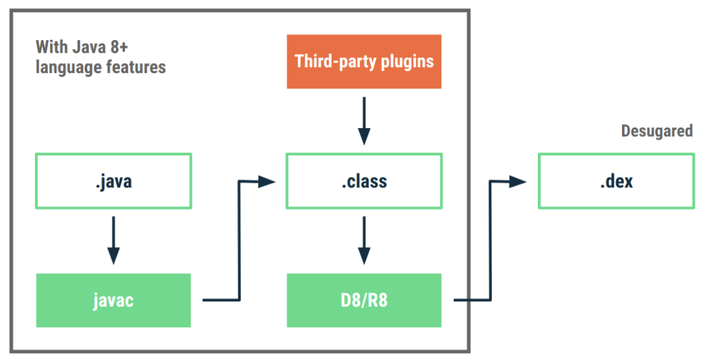
\includegraphics[width=0.8\textwidth]{images/javainandroid.png}
            \caption{Hỗ trợ tính năng ngôn ngữ Java 8 bằng cách desugar biến đổi mã byte \cite{java8}.}
            \label{fig:android2}
        \end{figure}
        
        Trình bổ trợ Android cho Gradle cung cấp khả năng hỗ trợ tích hợp để sử dụng một số tính năng ngôn ngữ Java 8 cùng các thư viện bên thứ ba sử dụng những tính năng đó. Chuỗi công cụ mặc định triển khai các tính năng ngôn ngữ mới bằng cách thực hiện các biến đổi mã byte(được gọi là desugar) như một phần của quá trình biên dịch các tệp lớp D8/R8 thành mã DEX, như minh hoạ trong hình \cite{java8}.


\section{Kết luận}
    Kiến trúc ứng dụng Android được thiết kế theo hướng mô-đun, phân tầng rõ ràng nhằm đảm bảo tính linh hoạt, dễ mở rộng và bảo mật cao. Ứng dụng Android chạy trên nền tảng hệ điều hành Android, vốn được xây dựng dựa trên nhân Linux – nơi chịu trách nhiệm quản lý phần cứng, tiến trình và bộ nhớ. Trên nền đó, Android triển khai nhiều cơ chế bảo mật như sandbox, UID riêng biệt, máy ảo(Dalvik hoặc ART), hệ thống phân quyền truy cập và SELinux để cô lập các ứng dụng, đảm bảo rằng mỗi ứng dụng chỉ hoạt động trong phạm vi tài nguyên được phép. Kiến trúc ứng dụng bao gồm nhiều thành phần như Activity, Service, BroadcastReceiver và ContentProvider, được khai báo trong file AndroidManifest.xml và quản lý bởi hệ thống Android Framework. Dữ liệu và mã nguồn được đóng gói trong tệp APK, trong đó có chứa bytecode .dex, tài nguyên biên dịch và thông tin cấu hình. Ngoài ra, Android còn hỗ trợ các công cụ hiện đại như Gradle, D8/R8, và quy trình desugaring để tương thích với các tính năng Java mới. Nhờ sự kết hợp giữa nền tảng Linux ổn định, mô hình máy ảo hiệu quả, cùng các lớp bảo mật chặt chẽ và công cụ phát triển mạnh mẽ, kiến trúc ứng dụng Android ngày càng hoàn thiện, tạo điều kiện thuận lợi cho lập trình viên xây dựng các ứng dụng hiệu suất cao và an toàn cho người dùng.\\

